% Sidebar subcategory icon: Sphere elements — two particles of DIFFERENT radius
% with their centre nodes marked: a one-node cell plus the RADIUS that is what
% makes it a sphere rather than a point. Distinct from `spheres` (an overlapping
% cluster with a radius line), the icon of the Set-element-radius form inside.
% NOTE: the committed svg-ui/catSpheres.svg was hand-authored to the same
% drawing (no pdftocairo available); regenerating via `make ui` replaces it with
% the pdftocairo rendering of this source — same glyph either way.
\documentclass[tikz,border=2mm]{standalone}
\usetikzlibrary{arrows.meta,calc,shapes.geometric}
\begin{document}
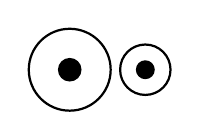
\begin{tikzpicture}[line width=1.3pt, line cap=round, line join=round, x=1mm,y=1mm]
  \draw[thick] (-3.2,0) circle (5.2);
  \draw[thick] (6.4,0) circle (3.2);
  \fill (-3.2,0) circle (1.5);           % centre nodes (the actual cells)
  \fill (6.4,0) circle (1.2);
\end{tikzpicture}
\end{document}
